\documentclass[../main.tex]{subfiles}
\begin{document}
\section{Výběr příznaků}

Často je výhodné počet příznaků před trénováním modelů snížit. Proces, který zvolí nějakou výhodnou podmnožinu příznaků, je feature selection. Tento proces spadá do části předzpracování dat, konkrétně se jedná o podoblast redukce dimenzionality (dimension reduction).

Výběrem příznaků řešíme hned několik problémů najednou:
\begin{itemize}
    \item Zahozením nerelevantních a redundantních příznaků můžeme významně zlepšit schopnost generalizace modelu (model není zatížený šumem).
    \item Pomáhá s prokletím dimenzionality (curse of dim.), kdy vysoká dimenze způsobuje řídkost dat a nerelevantnost sousedství.
    \item Zlepšuje interpretovatelnost modelu.
    \item Snižuje výpočetní nároky pro trénování.
\end{itemize}

\subsection{Základní metody výběru příznaků}

\subsubsection{Filtrační metody}

Filtrační metody jsou jednoduché a často nevyžadují náročné trénovaní modelů:
\begin{itemize}

    \item Vyhodit příznaky s příliš nízkým rozptylem (jsou téměř konstantní).

    \item Vyhodit příznaky, které mají příliš chybějících hodnot.

    \item Vyhodit redundantní příznaky, které mají vysokou korelaci s jiným příznakem (jsou v datasetu již zastoupeny).

    \item Vyhodit příznaky, které mají s cílovou proměnnou nízkou korelaci (je dobré v kombinaci s bázovými funkcemi -- samotný příznak totiž nemusí vysvětlovanou proměnnou ovlivňovat pouze lineárně).

    \item U binárních příznaků rozdělit data na dvě populace a provést hypotézu o rovnosti středních hodnot obou populací (dvouvýběrový t-test).

    \item Provést test nezávislosti mezi příznakem a vysvětlovanou proměnnou.

\end{itemize}

\subsubsection{Obalové metody}

Obalové metody používají pro ohodnocení příznaků pomocný model, který na příslušné kandidátní množině příznaků natrénují a pak výkon porovnají se stejným modelem natrénovaný na jiné sadě příznaků.

Pokud se jako pomocný model použije finální model, je výhodou, že se zvolí tu sadu příznaků, která dobře pracuje s vybraným modelem. V takovém případě však snadněji dochází k přeučení. Vybere-li se ale jiný model, sada příznaků může být zvolena nevýhodně pro finální model.

Pokud je kandidátních množin příznaků hodně, je tato metody výpočetně náročná, proto se často používají hladové algoritmy:
\begin{itemize}

    \item Dopředný výběr (forward selection) začíná s prázdnou množinou a postupně přidává příznak, který v dané iteraci nejvíce zvýší výkonnost modelu.

    \item Zpětný výběr (backward selection) začíná se všemi příznaky a postupně odebírá ty, které nejméně sníží výkonnost modelu.

    \item Rekurzivní odebírání příznaků (recursive feature elimination) postupně odebírá podle vnitřního ohodnocení příznaků pomocného modelu (u norm. lineární regrese koeficienty, u stromu příslušný informační zisk)

\end{itemize}
Algoritmy běží dokud nemají požadovaný počet příznaků, případně mohou skončit i s menším počtem příznaků, pokud přidávání, resp. odstranění, příznaků nesnižuje výkonnost.

\subsubsection{Vestavěné metody}

Vestavěné metody (embedded methods) provedou výběr příznaků natrénováním modelu na celých datech a pak zahodí příznaky, které se naučil vůbec nepoužívat.

U lineární regrese se jedná o příznaky s koeficientem 0, u rozhodovacího stromu ty, které se nikde nepoužily, atd.

\subsection{Lasso} \label{sec:lasso}

Nejpoužívanější vestavěnou metodou je $L_1$ regularizovaná lineární regrese, která volí množinu příznaků s nenulovým koeficientem.

Na rozdíl od hřebenové regrese penalizuje absolutní hodnotu koeficientů. Pro $\lambda \ge 0$ minimalizuje
\[
    \RSS_\lambda^\Lasso = \sum_{i=1}^{N} (Y_i - \hat{Y}_i)^2
    + \lambda \sum_{i=1}^{p} |w_i|
\]
Pro $\lambda = 0$ se jedná o klasickou lineární regresi. Pro $\lambda > 0$ cílí na co nejmenší koeficienty, ale nevadí mu vysoké hodnoty.

$\RSS_\lambda^\Lasso$ není diferencovatelný, proto se řešení hledá iterativní metodou:
\[
    \wh_\lambda^\Lasso = \argmin_{\we} \RSS_\lambda^\Lasso (\we)
\]
Výhoda modelu Lasso je, že $\wh_\lambda^\Lasso$ je řídké -- hodně členů je rovno nule. S vyšší $\lambda$ jsou nuly častější.

Formální důkaz tohoto tvrzení je složitý, ale pro představu lze znázornit obrázkem.

\begin{center}
    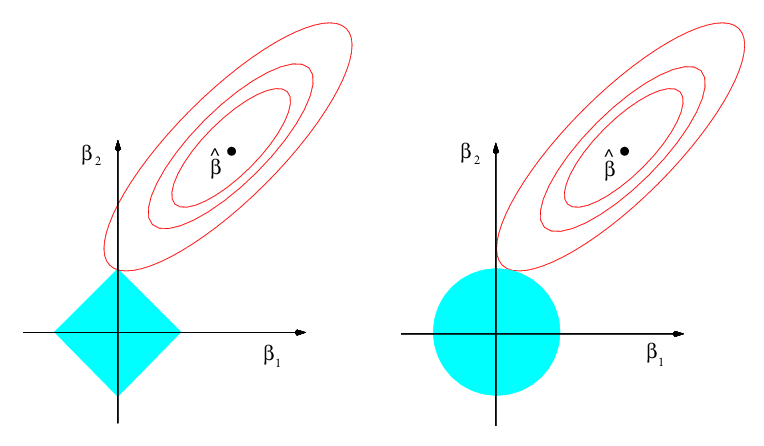
\includegraphics[width=12cm]{lasso}
\end{center}

Červeně jsou vykreslené vrstevnice parabolické jámy neregularizované části ${\sum_{i=1}^{N} (Y_i - \hat{Y}_i)^2}$. Přímo na nějakých osách bude hyperkrychle vrstevnici protínat celkem často, zatímco hypersféra prakticky nikdy (pokud neleží minimum přimo na ose).

U Lasso může být nežádoucí, že v případě kolinearity má tendenci volit pouze některé z příznaků. To se projevuje jako nevýhoda především u nových dat -- příznak může chybět nebo být sám o sobě zatížený nějakým šumem. Proto existuje model, elastic net, který má oba regularizační členy ($L_1$ i $L_2$) a kombinuje výhody obou přístupů:
\[
    \RSS_{\lambda_1, \lambda_2}^\Elastic = \sum_{i=1}^{N} (Y_i - \hat{Y}_i)^2
    + \lambda_1 \sum_{i=1}^{p} |w_i|
    + \lambda_2 \sum_{i=1}^{p} w_i^2
\]
\[
    \wh_{\lambda_1, \lambda_2}^\Elastic
    = \argmin_{\we} \RSS_{\lambda_1, \lambda_2}^\Elastic (\we)
\]

\end{document}
